% SOLO P2
% Todos los valores provienen de las tablas de resultados/ que generan los notebooks
% P03, P04 y P05; las figuras se generan con paper/generar_figuras.py.
\section{Resultados y análisis}
\label{sec:resultados}

\subsection{Selección de hiperparámetros}
La Fig.~\ref{fig:busqueda} resume la búsqueda en validación para las configuraciones con ponderación
de clases.

\begin{figure*}[t]
    \centering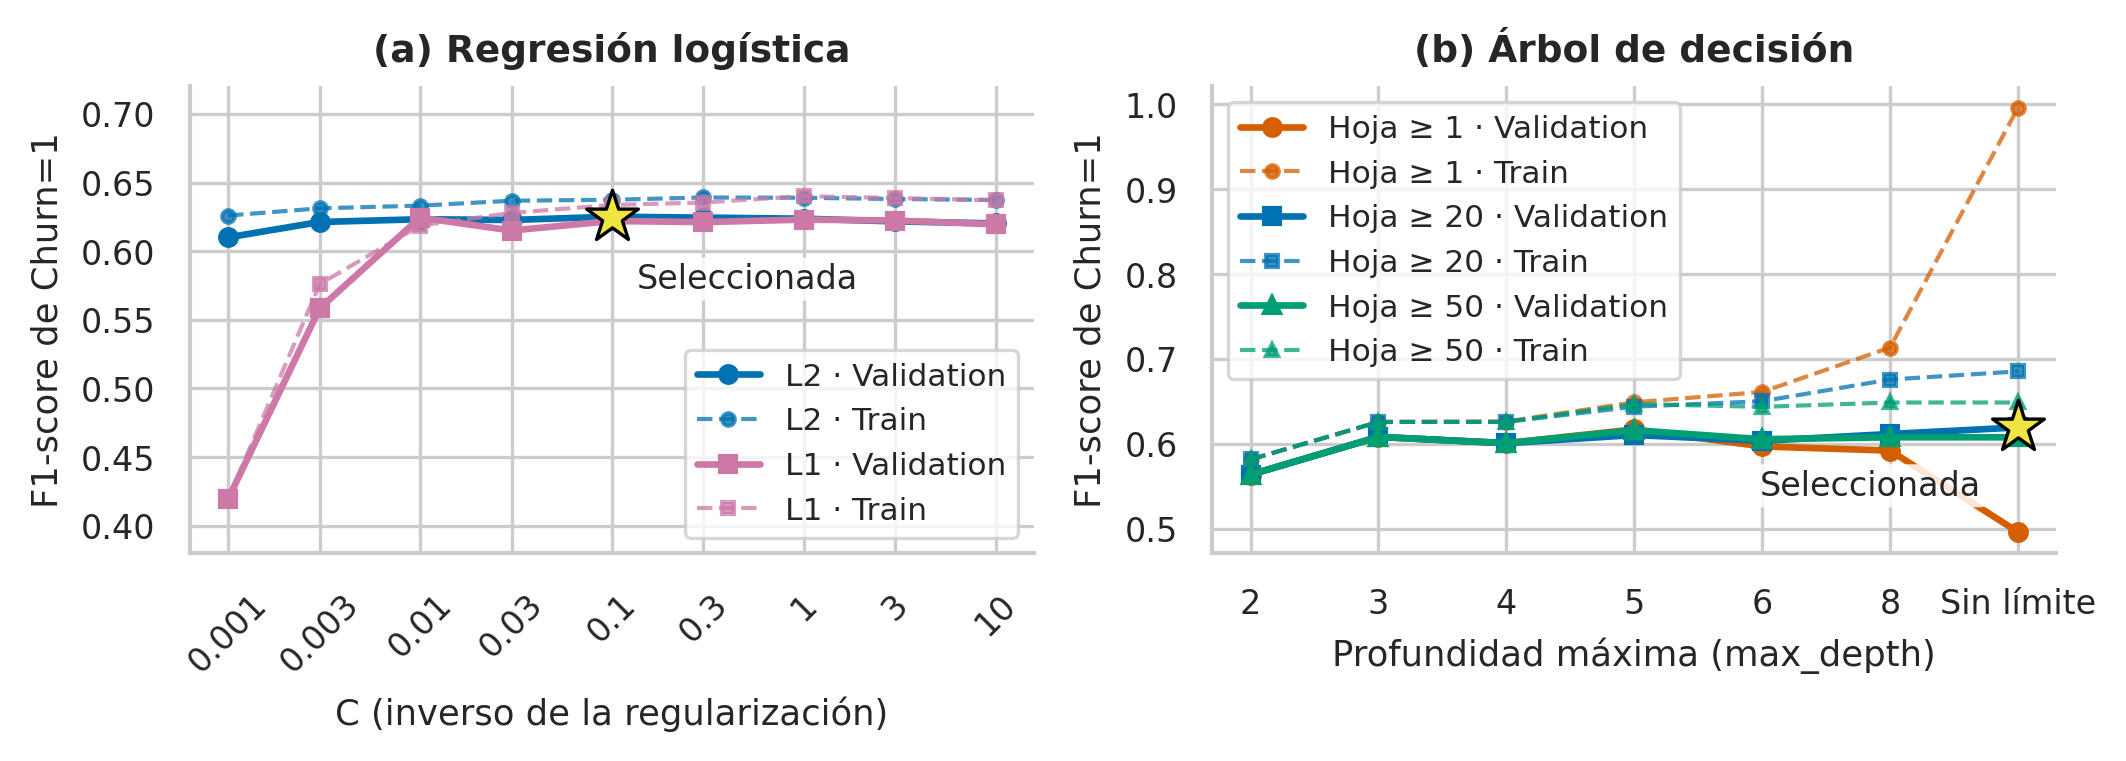
\includegraphics[width=\textwidth]{busqueda_hiperparametros.png}
    \caption{F1-score de \var{Churn=1} en entrenamiento (línea discontinua) y en validación (línea
    continua) para las configuraciones con \var{class\_weight=\textquotedbl{}balanced\textquotedbl{}}. (a) Regresión logística
    según $C$ y la penalización. (b) Árbol de decisión según la profundidad máxima y el tamaño mínimo
    de hoja. La estrella indica la configuración seleccionada.}
    \label{fig:busqueda}
\end{figure*}

En la regresión logística, la fuerza de la regularización importa poco fuera de los extremos: con L2
y ponderación, el F1 varía entre 0.610 y 0.625 en todo el rango de $C$, y las cinco mejores
configuraciones difieren en menos de 0.002. Se seleccionó L2 con $C$ = 0.1 y ponderación de clases
(F1 = 0.625). El F1 en entrenamiento es 0.637, a solo 0.012 del de validación, por lo que no hay
señales de sobreajuste. Con L1 y $C$ = 0.01 se obtiene prácticamente el mismo F1 (0.624) con solo 7 de
los 46 coeficientes distintos de cero: la señal se concentra en pocas variables.

Lo que sí cambia el resultado es el tratamiento del desbalance. Sin ponderación, la mejor
configuración alcanza F1 = 0.593, con \emph{Precision} 0.66 y \emph{Recall} 0.53. Con ponderación, el
\emph{Recall} sube a 0.79 a cambio de una \emph{Precision} de 0.52: el modelo detecta a muchos más
clientes que abandonan, pero genera más alertas falsas.

En el árbol, la decisión central es el control del sobreajuste. Sin restricciones, el árbol
ponderado crece hasta 859 hojas y alcanza F1 = 0.996 en entrenamiento, pero solo 0.496 en
validación: memoriza los datos. Al exigir al menos 20 clientes por hoja, el árbol se reduce a 132
hojas y 12 niveles y obtiene el mejor F1 de la grilla (0.619), con una brecha entre entrenamiento y
validación de 0.066. Esa es la configuración seleccionada. Árboles mucho más pequeños quedan muy
cerca: 0.617 con profundidad 5 (30 hojas) y 0.608 con profundidad 3 (8 hojas). La diferencia de F1
entre el árbol seleccionado y el de 8 hojas es 0.011, con intervalo bootstrap del 95\%
[$-$0.014, 0.035], es decir, no se distingue de cero. Se mantuvo la configuración que indica el
criterio fijado de antemano, aunque un árbol de 8 hojas habría sido casi igual de bueno y mucho más
fácil de leer. Como en la regresión logística, la ponderación es necesaria: el mejor árbol sin
ponderar llega a F1 = 0.579.

\subsection{Desempeño en el conjunto de prueba}
La Tabla~\ref{tab:test} presenta la evaluación final, realizada una sola vez.

\begin{table*}[t]
    \caption{Desempeño en el conjunto de prueba (1409 clientes, 374 abandonos). Entre corchetes,
    intervalo bootstrap del 95\%. Las cuatro últimas columnas son los conteos de la matriz de confusión}
    \label{tab:test}
    \centering\footnotesize
    \setlength{\tabcolsep}{3pt}
    \begin{tabular}{@{}lcccccrrrr@{}}
        \toprule
        Modelo & Accuracy & Precision & Recall & F1-score & ROC-AUC & VN & FP & FN & VP \\
        \midrule
        Referencia (\emph{Dummy}) & 0.735 [0.711, 0.759] & 0.000 & 0.000 & 0.000 & 0.500 & 1035 & 0 & 374 & 0 \\
        Regresión logística & 0.743 [0.720, 0.766] & 0.510 [0.470, 0.551] & 0.781 [0.736, 0.820]
        & 0.617 [0.579, 0.654] & 0.841 [0.818, 0.863] & 755 & 280 & 82 & 292 \\
        Árbol de decisión & 0.744 [0.720, 0.765] & 0.512 [0.469, 0.554] & 0.722 [0.675, 0.767]
        & 0.599 [0.559, 0.635] & 0.818 [0.793, 0.841] & 778 & 257 & 104 & 270 \\
        \bottomrule
    \end{tabular}
\end{table*}

El clasificador de referencia acierta en el 73.5\% de los clientes sin detectar ningún abandono. La
regresión logística detecta 292 de los 374 abandonos (\emph{Recall} = 0.781) y el árbol, 270
(0.722). En ambos, cerca de la mitad de las alertas corresponde a clientes que realmente abandonan
(\emph{Precision} $\approx$ 0.51), casi el doble de la tasa base de 26.5\%.

La exactitud de los dos modelos (0.743 y 0.744) no se distingue de la del clasificador de
referencia: la diferencia es de 0.009 en ambos casos, con intervalos [$-$0.025, 0.041] y
[$-$0.023, 0.040]. Esto no significa que los modelos no aporten, sino que la exactitud no mide lo que
interesa: los modelos cambian aciertos sobre clientes que permanecen por aciertos sobre clientes que
abandonan. Entre validación y prueba, el F1 baja de 0.625 a 0.617 en la regresión logística y de
0.619 a 0.599 en el árbol. Son caídas pequeñas frente a esos intervalos.

Al comparar los dos modelos sobre los mismos clientes, la regresión logística supera al árbol en
\emph{Recall} (+0.059, intervalo [0.016, 0.103]) y en ROC-AUC (+0.023 [0.009, 0.040]). En F1
(+0.018 [$-$0.009, 0.049]), \emph{Precision} y \emph{Accuracy} los intervalos incluyen el cero, así
que esas diferencias no son concluyentes. La Fig.~\ref{fig:curvas} muestra que la ventaja en ROC-AUC
no depende del umbral elegido: la curva de la regresión logística queda por encima de la del árbol en
casi todo el rango.

\begin{figure}[t]
    \centering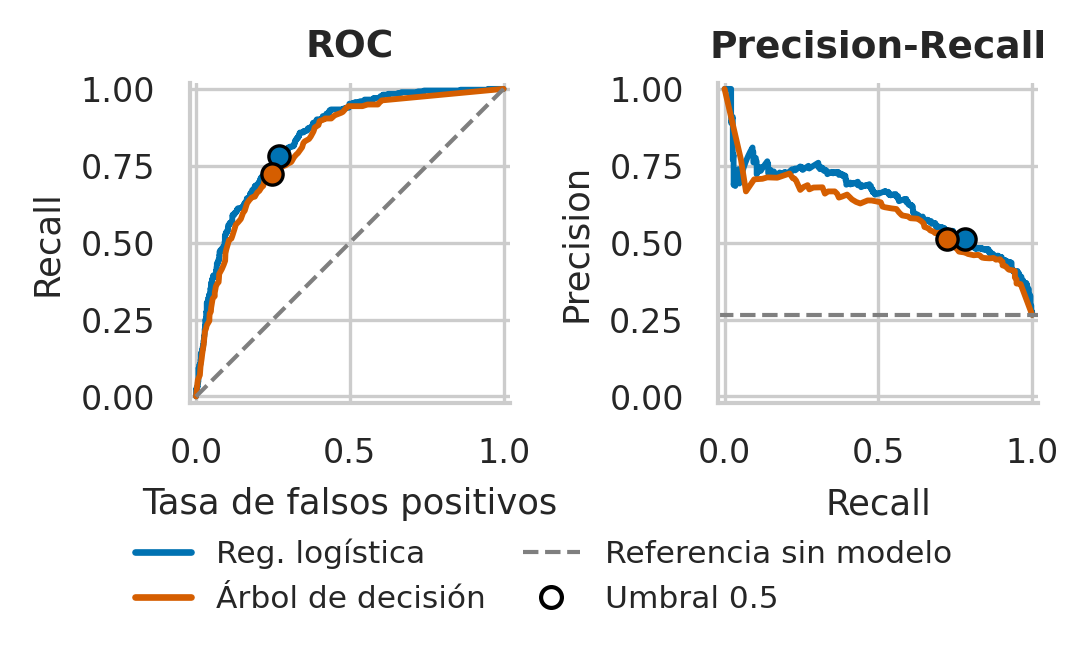
\includegraphics[width=\columnwidth]{curvas_roc_pr.png}
    \caption{Curvas ROC y Precision-Recall en el conjunto de prueba. Los puntos marcan el umbral 0.5
    usado para clasificar.}
    \label{fig:curvas}
\end{figure}

\subsection{Interpretación de los modelos}
\textbf{Regresión logística.} La Tabla~\ref{tab:odds} presenta las principales razones de \emph{odds} (OR)
obtenidas mediante contrastes entre perfiles hipotéticos del modelo, tomando como referencia la categoría más
frecuente de cada variable. Un contrato de dos años multiplica los \emph{odds} estimados de abandono por
0.24 frente al contrato mensual, mientras que no tener internet los multiplica por 0.19 frente a tener fibra
óptica. Doce meses adicionales de antigüedad, manteniendo el cargo mensual y ajustando el cargo acumulado, los
multiplican por 0.69. En contraste, el género (OR = 1.05) presenta una asociación estimada pequeña.

Estas direcciones son consistentes con los patrones del EDA, pero no representan efectos causales. En particular,
el OR de no tener telefonía (1.90) debe interpretarse con cautela, pues corresponde a una comparación condicionada
a las demás características del perfil. Se reportan contrastes entre categorías en lugar de interpretar
coeficientes aislados debido a las dependencias entre columnas generadas mediante \emph{one-hot encoding}.
Aunque la regularización L2 permite obtener una solución única de coeficientes, los contrastes ofrecen una
interpretación más útil bajo esta representación redundante.

\begin{table}[t]
    \caption{Razones de \emph{odds} de la regresión logística respecto de la categoría de referencia}
    \label{tab:odds}
    \centering\footnotesize
    \begin{tabular}{@{}llr@{}}
        \toprule
        Variable & Contraste & OR \\
        \midrule
        \var{InternetService} & No frente a Fiber optic & 0.19 \\
        \var{Contract} & Two year frente a Month-to-month & 0.24 \\
        \var{Contract} & One year frente a Month-to-month & 0.46 \\
        \var{InternetService} & DSL frente a Fiber optic & 0.50 \\
        \var{PhoneService} & No frente a Yes & 1.90 \\
        \var{OnlineSecurity} & Yes frente a No & 0.66 \\
        \var{PaymentMethod} & Bank transfer frente a Electronic check & 0.68 \\
        \var{TechSupport} & Yes frente a No & 0.69 \\
        \var{SeniorCitizen} & 1 frente a 0 & 1.18 \\
        \var{gender} & Female frente a Male & 1.05 \\
        \midrule
        \var{tenure} & +12 meses, mismo cargo mensual & 0.69 \\
        \var{MonthlyCharges} & +20 USD durante toda la antigüedad & 1.20 \\
        \bottomrule
    \end{tabular}
\end{table}

\textbf{Árbol de decisión.} La Fig.~\ref{fig:arbol} muestra los dos primeros niveles del árbol
seleccionado. La primera pregunta es si el contrato es mensual: entre quienes no lo tienen, la tasa
de abandono en entrenamiento es 6.3\%; entre quienes sí, 43.1\%. Dentro del contrato mensual, la
segunda pregunta es el tipo de internet: con fibra óptica la tasa sube a 55.5\% y, en el nivel
siguiente, a 69.4\% cuando además la antigüedad no supera los 15 meses. Cada hoja predice abandono
cuando su tasa en entrenamiento supera la tasa global de 26.5\%, que es el efecto de la ponderación
de clases; 58 de las 132 hojas lo hacen. El árbol completo no se puede leer como un conjunto corto de
reglas, pero sus primeros niveles sí.

\begin{figure}[t]
    \centering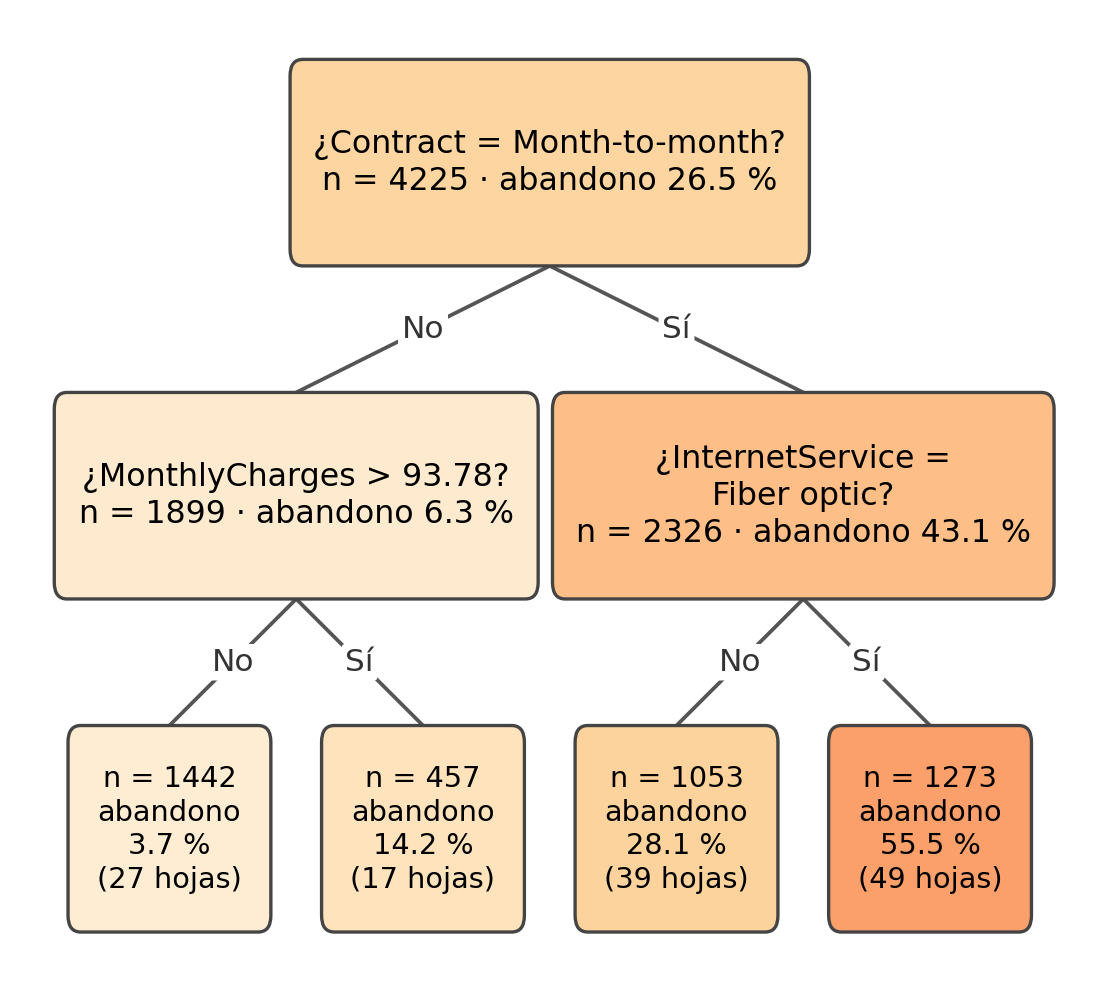
\includegraphics[width=\columnwidth]{arbol_primeros_niveles.png}
    \caption{Primeros dos niveles del árbol seleccionado, con el número de clientes y la tasa de
    abandono observada en entrenamiento. Las cajas inferiores resumen el subárbol que cuelga de cada
    una.}
    \label{fig:arbol}
\end{figure}

\textbf{Importancia por permutación.} La Fig.~\ref{fig:importancia} compara ambos modelos en la
misma escala. Los dos dependen de las mismas tres variables, \var{Contract}, \var{tenure} e
\var{InternetService}, aunque con distinto reparto: la regresión logística se apoya sobre todo en
\var{tenure} (el F1 cae 0.126 al desordenarla) y el árbol en \var{Contract} (0.180) e
\var{InternetService} (0.138). Las demás variables aportan mucho menos, y \var{gender} no aporta de
forma medible en ninguno. 
La importancia individual puede subestimarse ante predictores correlacionados, como \var{tenure} y
\var{TotalCharges}. Además, la permutación independiente de variables relacionadas puede generar combinaciones
poco posibles, por lo que estos valores deben interpretarse como medidas de dependencia predictiva
bajo la perturbación aplicada, no como efectos causales.

\begin{figure}[t]
    \centering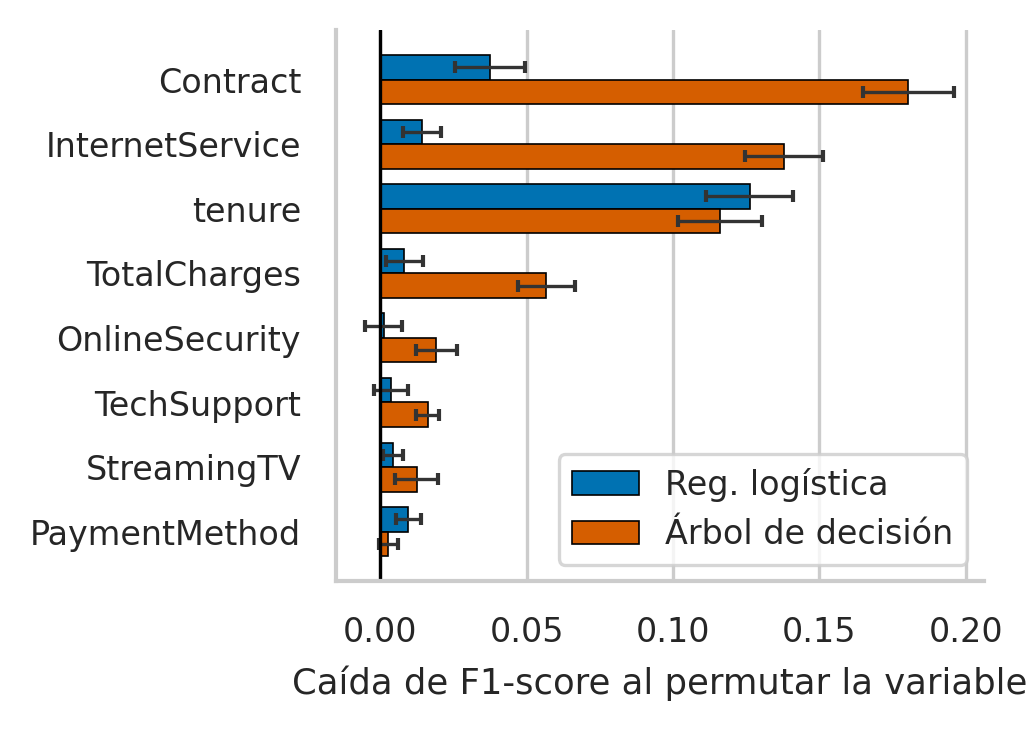
\includegraphics[width=\columnwidth]{importancia_permutacion.png}
    \caption{Importancia por permutación en validación: caída media del F1-score al desordenar cada
    variable (30 repeticiones; las barras de error indican una desviación estándar). Se muestran las
    ocho variables con mayor importancia.}
    \label{fig:importancia}
\end{figure}

\subsection{Análisis de errores}
\label{sec:errores}
Los errores no se reparten al azar. La Tabla~\ref{tab:subgrupos} muestra el \emph{Recall} y la tasa
de falsos positivos (TFP, proporción de clientes que permanecen y reciben una alerta) por subgrupo.

\begin{table}[t]
    \caption{\emph{Recall} y tasa de falsos positivos (TFP) por subgrupo en prueba. RL: regresión
    logística; AD: árbol de decisión; Ab.: abandonos}
    \label{tab:subgrupos}
    \centering\footnotesize
    \setlength{\tabcolsep}{3.5pt}
    \begin{tabular}{@{}lrrcccc@{}}
        \toprule
        & & & \multicolumn{2}{c}{Recall} & \multicolumn{2}{c}{TFP} \\
        \cmidrule(lr){4-5}\cmidrule(l){6-7}
        Subgrupo & $n$ & Ab. & RL & AD & RL & AD \\
        \midrule
        \multicolumn{7}{@{}l}{\emph{Contrato}} \\
        Month-to-month & 773 & 329 & 0.863 & 0.809 & 0.595 & 0.550 \\
        One year & 300 & 36 & 0.222 & 0.111 & 0.061 & 0.049 \\
        Two year & 336 & 9 & 0.000 & 0.000 & 0.000 & 0.000 \\
        \multicolumn{7}{@{}l}{\emph{Antigüedad (meses)}} \\
        0--12 & 449 & 215 & 0.842 & 0.842 & 0.538 & 0.513 \\
        13--24 & 206 & 60 & 0.883 & 0.733 & 0.486 & 0.384 \\
        25--48 & 304 & 64 & 0.688 & 0.516 & 0.250 & 0.183 \\
        49--72 & 450 & 35 & 0.400 & 0.343 & 0.055 & 0.089 \\
        \multicolumn{7}{@{}l}{\emph{Servicio de internet}} \\
        Fiber optic & 613 & 252 & 0.905 & 0.810 & 0.535 & 0.468 \\
        DSL & 484 & 97 & 0.660 & 0.567 & 0.222 & 0.173 \\
        No & 312 & 25 & 0.000 & 0.440 & 0.003 & 0.073 \\
        \multicolumn{7}{@{}l}{\emph{SeniorCitizen}} \\
        0 & 1187 & 276 & 0.728 & 0.688 & 0.243 & 0.226 \\
        1 & 222 & 98 & 0.929 & 0.816 & 0.476 & 0.411 \\
        \multicolumn{7}{@{}l}{\emph{Género}} \\
        Female & 687 & 193 & 0.782 & 0.715 & 0.271 & 0.255 \\
        Male & 722 & 181 & 0.779 & 0.729 & 0.270 & 0.242 \\
        \bottomrule
    \end{tabular}
\end{table}

Ambos modelos concentran sus alertas en los perfiles que el EDA asoció con mayor abandono. En el
contrato mensual detectan más del 80\% de los abandonos, pero también señalan a más de la mitad de
los clientes que permanecen. En el extremo opuesto, ninguno detecta a los 9 clientes con contrato de
dos años que abandonaron, y con contrato anual detectan como máximo 8 de 36. Lo mismo ocurre con la
antigüedad: el \emph{Recall} no pasa de 0.40 entre quienes llevan más de 48 meses. Entre los
clientes sin internet, la regresión logística no detecta ninguno de los 25 abandonos y el árbol
detecta 11. Por género prácticamente no hay diferencias. En cambio, entre los adultos mayores
(\var{SeniorCitizen=1}) el \emph{Recall} es más alto, pero la tasa de falsos positivos es
casi el doble que en el resto.

Los dos modelos se equivocan, en gran parte, con los mismos clientes: coinciden en la predicción del
84.7\% de los casos, 249 de los 374 abandonos (66.6\%) son detectados por ambos y 61 (16.3\%) por
ninguno. Los abandonos que la regresión logística no detecta tienen una antigüedad mediana de 26
meses, frente a 6 en los detectados, y solo el 54.9\% tiene contrato mensual, frente al 97.3\%. Es
decir, son clientes que abandonan con un perfil parecido al de quienes permanecen. Las falsas alarmas
son el caso inverso: el 94.3\% tiene contrato mensual y el 68.9\% fibra óptica.

Por último, las probabilidades estimadas no están calibradas. En prueba, su media es 0.414 en la
regresión logística y 0.389 en el árbol, frente a una tasa real de 0.265.
La ponderación de clases puede contribuir a esta sobreestimación, aunque no permite explicar por sí
sola toda la diferencia. Por ello, las puntuaciones resultan útiles para ordenar clientes según el
riesgo estimado y aplicar el umbral de clasificación, pero no deben interpretarse directamente como
probabilidades reales de abandono sin una evaluación y calibración adicionales.
